%====================================================================================================
\chapter{Development of a Simulator for L0 Endcap Muon Trigger System} \label{ch:L0MuonS1TGC}
%====================================================================================================
This chapter presents the development of a simulator for the TGC Sector Logic, which performs the trigger behavior on the endcap region of L0 muon trigger system. This simulator, so called L0MuonS1TGC simulator, is for a detailed and precise simulation, based on an existing bit-level simulator called "bitwise simulator" which emulates the firmware of TGC sector logic. The chapter begins by describing the structure and logic of the original bitwise simulator, including its hit processing and reconstruction pipeline. It then introduces the local implementation of this simulator within the ATLAS software framework, Athena, enabling simulation with full endcap part of detector geometry. Finally, it discusses the memory optimization techniques applied to the Look-Up Tables (LUTs) achieved as a preparation for implementation on Athena itself.
%====================================================================================================
\section{Bitwise Simulator} \label{sec:BitwiseSimulator}
%====================================================================================================
The bitwise simulator is a C++-based software tool developed for the Phase-II upgrade that emulates the TGC Sector Logic (SL) by replicating the bitwise operations performed by the hardware. It received hit map of wire segment and strip segment as input, then reconstruct the muon tracks and output the position information ($\eta$, $\phi$) and the transverse momentum ($p_\mathrm{T}$) to the next trigger process module. Figure~\ref{fig:blockDiagram} shows the block diagram of the trigger logic of the endcap SL firmware. The firmware consists of four Super Logic Regions (SLRs) on FPGAs. Among them, SLR0, SLR2, and SLR3 are simulated by the bitwise simulator to reconstruct muon candidates in the Endcap 1, Endcap 2, and Forward regions, respectively, as illustrated in Figure~\ref{fig:endcapAndForward}. SLR1 functions as a post-processing stage for the other three SLRs, forwarding the reconstructed results to the Inner Coincidence module in order to suppress muons that do not originate from the initial proton-proton collision point.
TrackSelector selects muon candidates with higher $p_\mathrm{T}$ and forwards them to the \MUCTPI for trigger processing.
\begin{figure}[htbp]
  \centering
  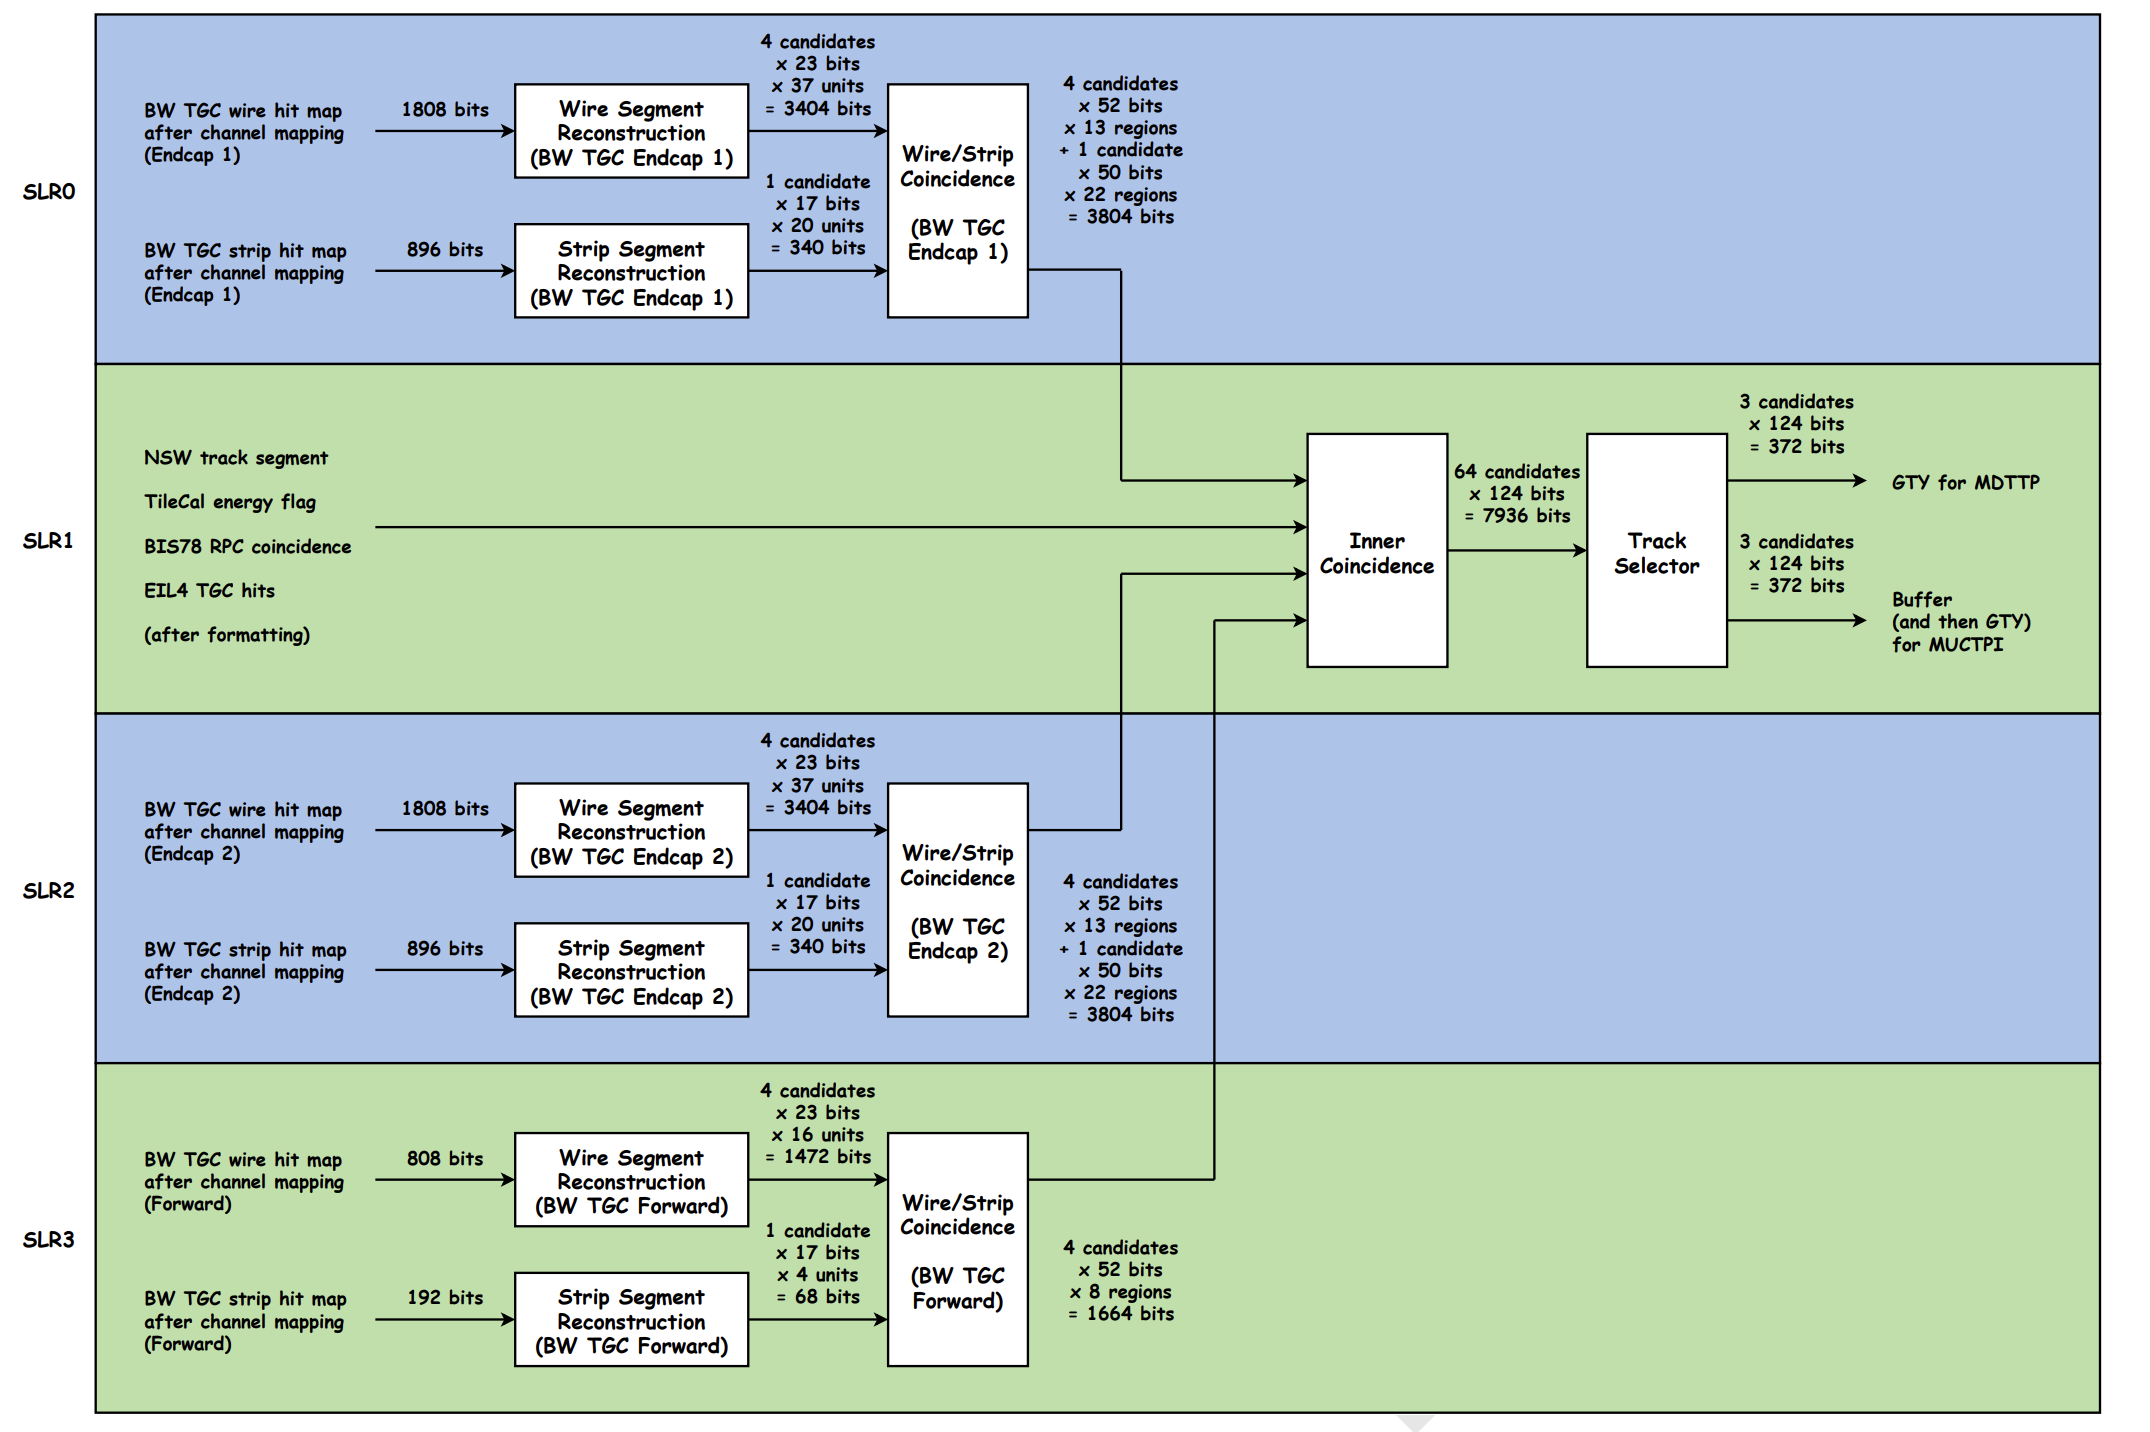
\includegraphics[width=1\textwidth]{figs/chapter5/block_diagram_of_trigger_logic.png}
  \caption{Block diagram of the Trigger Logic of the Endcap SL firmware \cite{EndcapSLPDR}.}
  \label{fig:blockDiagram}
\end{figure}

\begin{figure}[htbp]
  \centering
  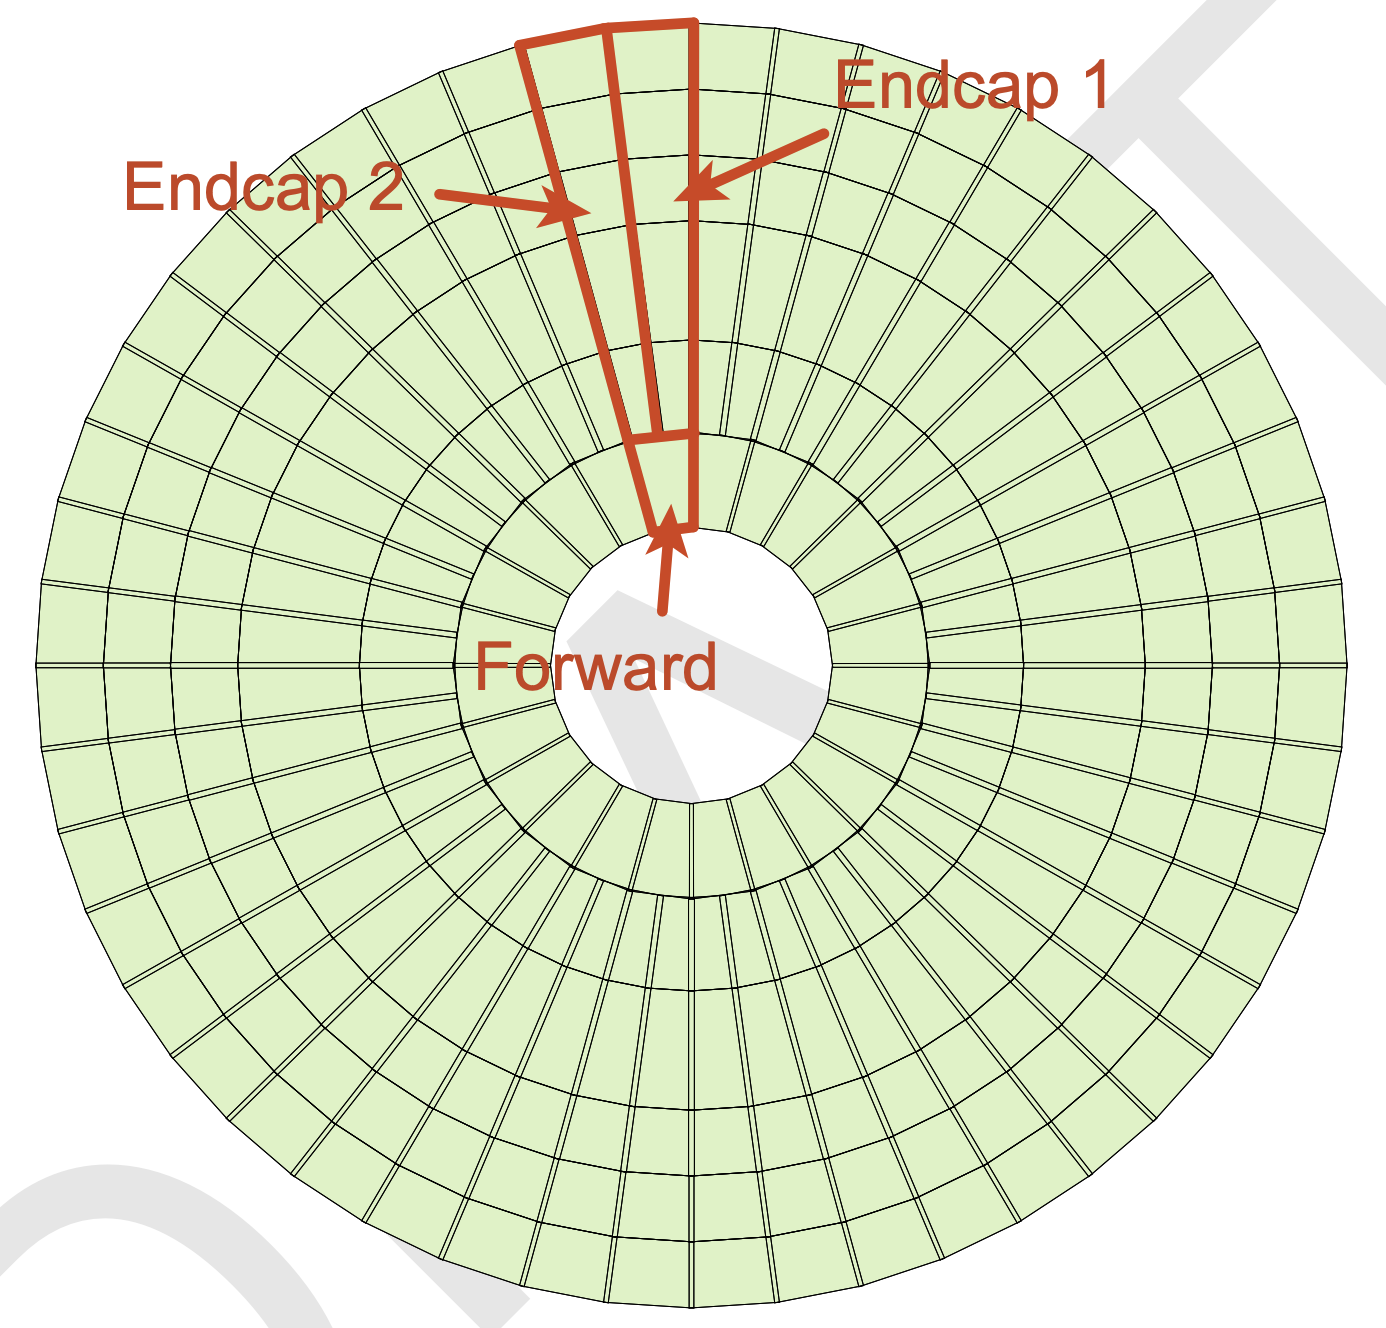
\includegraphics[width=0.8\textwidth]{figs/chapter5/endcap_and_forward_region.png}
  \caption{Schematic view of Big Wheel (\BW) TGC of an Endcap \SL blade, which is segmented into the "Endcap 1", "Endcap 2", and Forward trigger sectors \cite{EndcapSLPDR}.}
  \label{fig:endcapAndForward}
\end{figure}

%====================================================================================================
\subsection{Channel Mapping} \label{subsec:ChannelMapping}
%====================================================================================================
Each \SL corresponds to one of the 1/24 repetitive segments of the TGC Big Wheel (\BW). And each SL board receives hit information from 29 Primary Processor boards (\PS boards) in the previous stage via two optical links. Each link transmits 128 bits of data every 25 ns, resulting in a complete input to the Sector Logic in the form of a 128-bit $\times$ 58-link bitmap。

As the first stage of the bitwise simulator, the Channel Mapping module is responsible for converting this 128 $\times$ 58 bitmap input—originating from the \PS boards—into a format suitable for the next processing stage, the Intra-Station Coincidence. This conversion process is referred to as \textit{mapping}. During this step, the original bitmap is transformed into a well-structured, intuitive, three-dimensional vector format that reflects the geometrical structure of the TGC detector. Each hit is represented by a tuple of subsector, layer, and channel, uniquely identifying its position within the detector. This structured representation enables efficient coincidence detection across different layers within the same station in the subsequent logic stage.
%====================================================================================================
\subsection{Intra Station Coincidence} \label{subsec:IntraCoin}
%====================================================================================================
As described in Section~\ref{sec:TGC}, in order to achieve higher position resolution, the detector channels within each of the three TGC stations are deliberately staggered relative to the adjacent layers. The Intra-Station Coincidence step reorganizes the hits detected by each layer within a station according to predefined coincidence types. This process yields a Position ID (also referred to as a staggered ID), which is stored in vector form and serves as the input for Segment Reconstruction.
Figure~\ref{fig:IntraCoin} illustrates an example of the reconstruction method for Intra-Station Coincidence in the M1 station of a TGC Wire segment.

\begin{figure}[htbp]
  \centering
  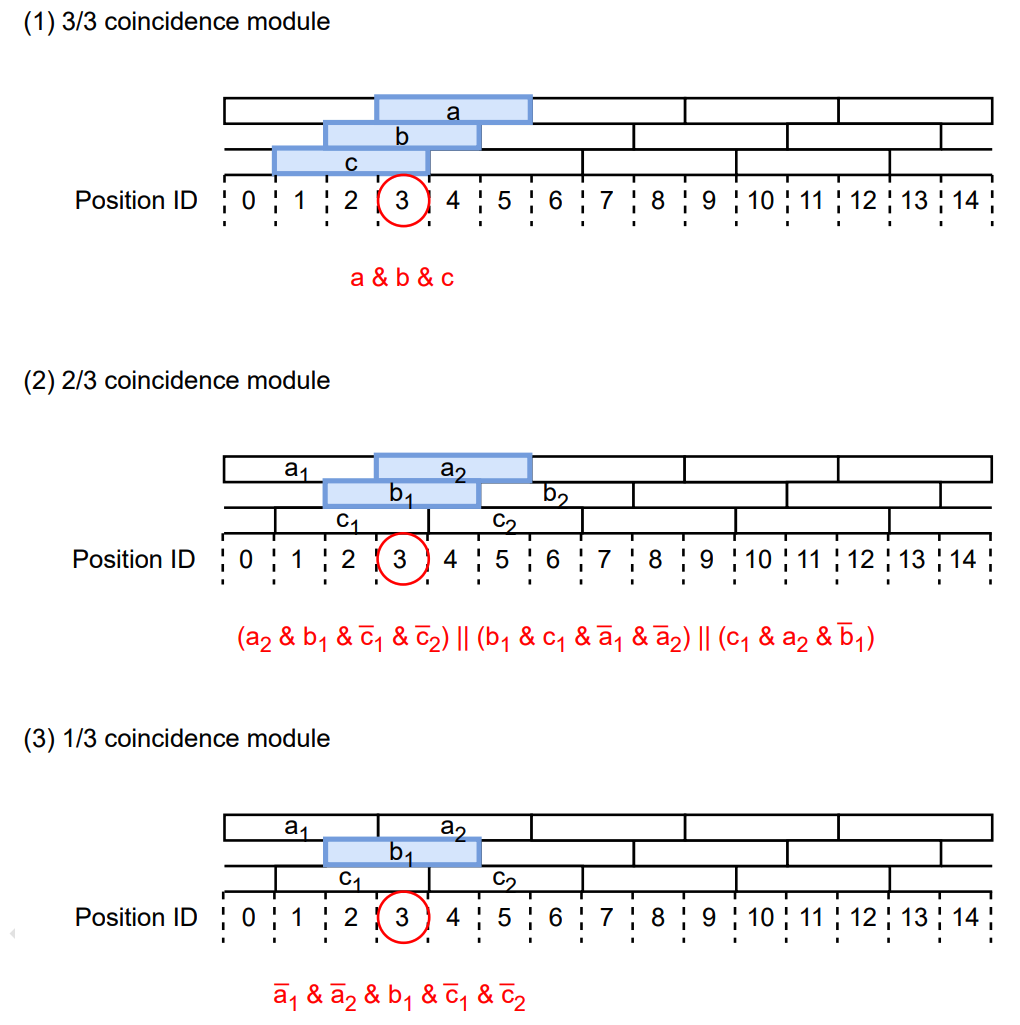
\includegraphics[width=0.8\textwidth]{figs/chapter5/Intra_station_coincidence.png}
  \caption{Concept of the station coincidence for TGC wire channels in M1 (triplet) \cite{EndcapSLPDR}.}
  \label{fig:IntraCoin}
\end{figure}

For the Phase-II upgrade, a more flexible coincidence logic has been adopted compared to that of Run 3 (see \cite{yamashita}).
%====================================================================================================
\subsection{Segment Reconstruction} \label{subsec:SegRec}
%====================================================================================================
Using the combination of Position IDs calculated from the three stations M1, M2, and M3 in the previous step, a pre-calculated Look-Up Table (LUT) is queried to obtain the corresponding deviations from an infinite-momentum trajectory, denoted as $\Delta\theta$ (for wires) and $\Delta\phi$ (for strips), as illustrated in Figure~\ref{fig:EndcapTriggerLogic}. These values, $\Delta\theta$ and $\Delta\phi$, represent the curvature of the muon’s trajectory under the influence of the toroidal magnetic field within the detector, with the position information of hits, are passed to the subsequent Wire-Strip Coincidence process for momentum calculation.

\begin{figure}[htbp]
  \centering
  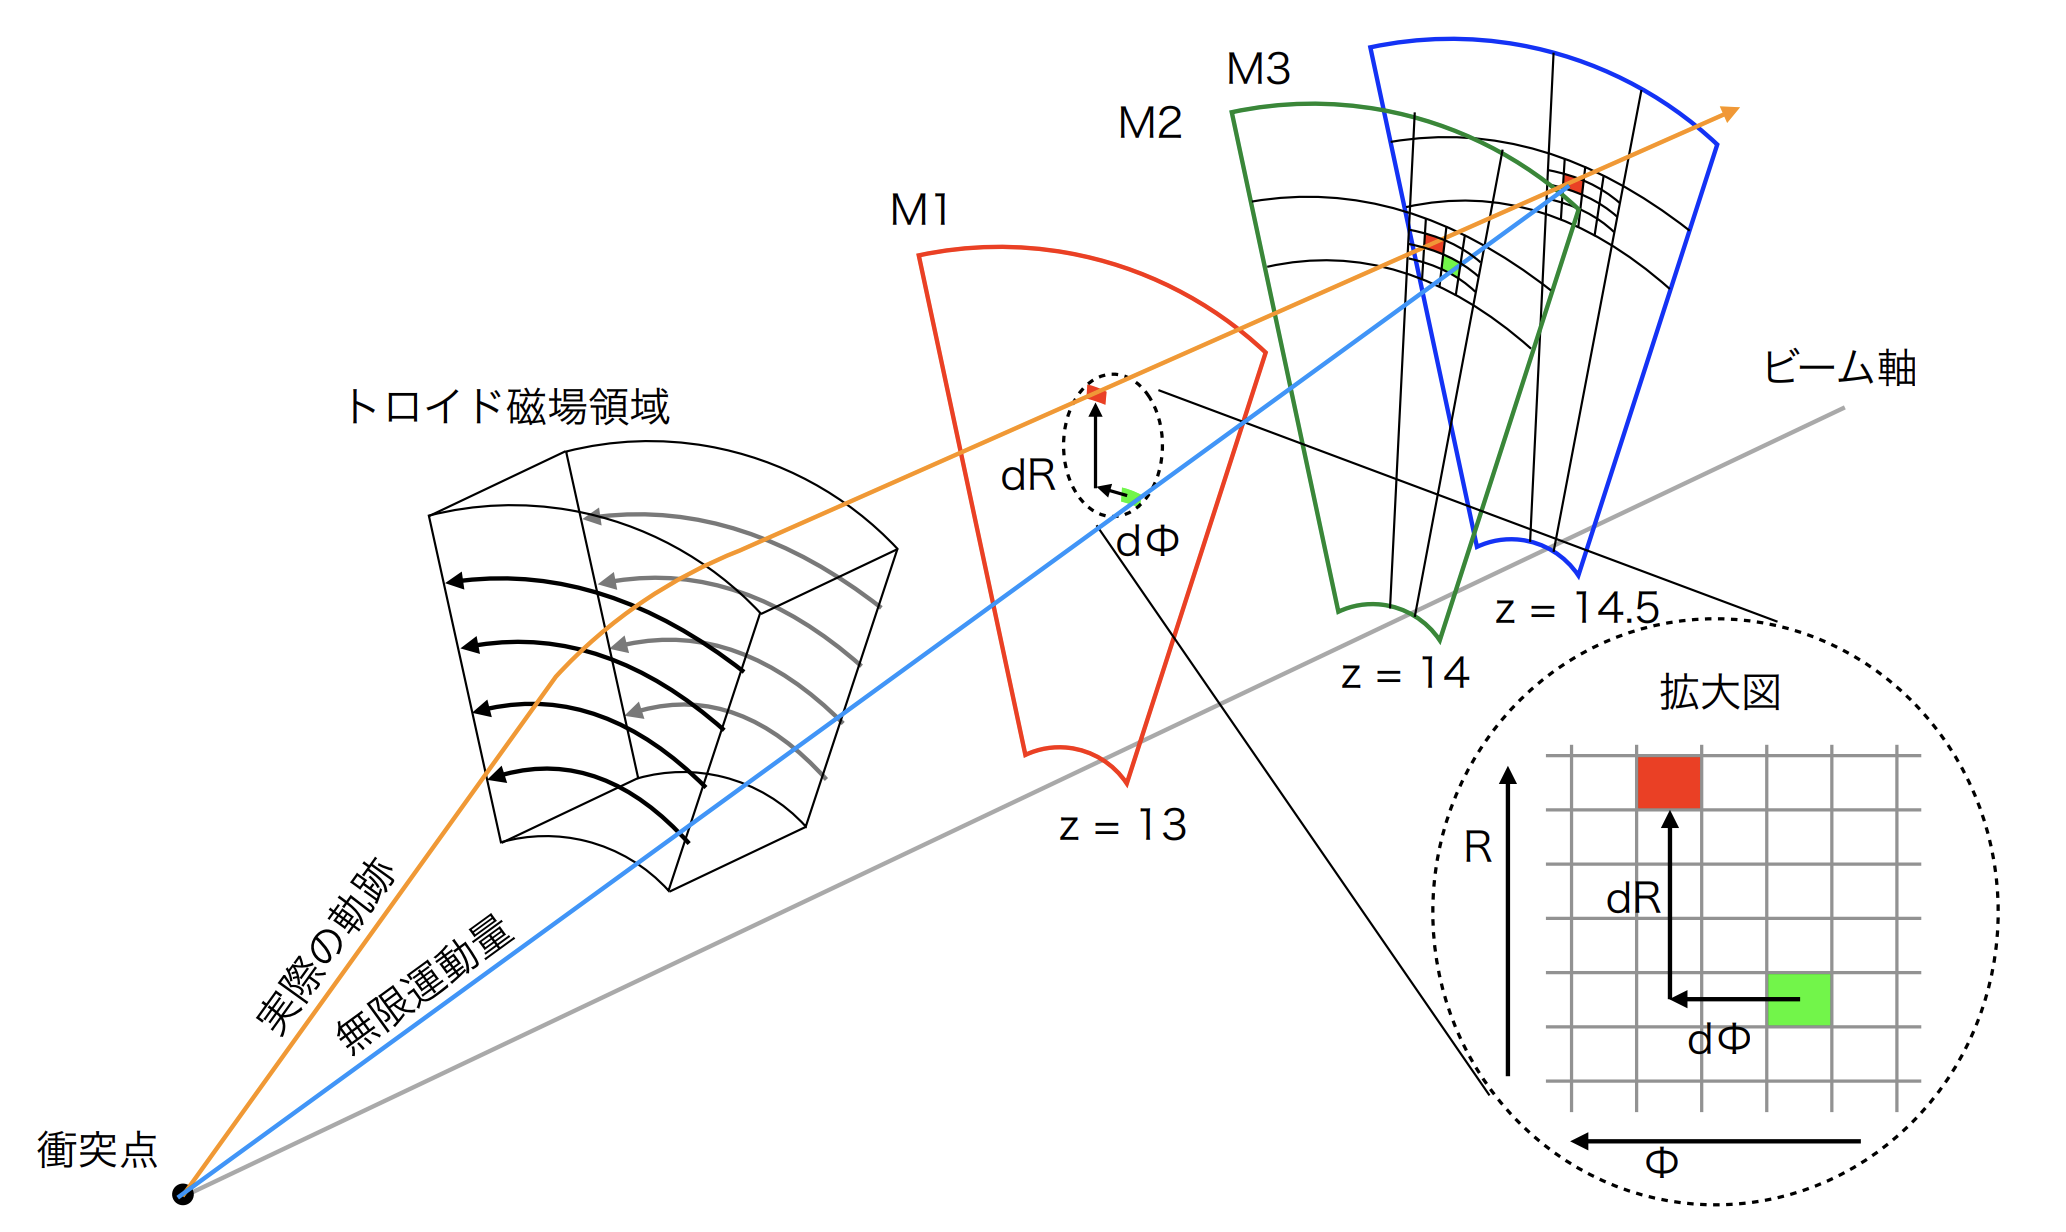
\includegraphics[width=0.8\textwidth]{figs/chapter5/endcap_trigger_logic_concept.png}
  \caption{Reconstruction logic of the endcap muon trigger. Note that the quantity labeled as \textit{dR} in the figure corresponds to $\Delta\theta$ in the coordinate system used in this paper \cite{akatsuka}.}
  \label{fig:EndcapTriggerLogic}
\end{figure}

The LUT is preloaded with possible combinations of Position IDs and their corresponding $\Delta\theta$ and $\Delta\phi$ values to eliminate redundant computations and accelerate the reconstruction process. In the firmware, the LUT is accessed via UltraRAM (URAM), a form of high-speed random-access memory. While in the bitwise simulator, this functionality is emulated using a \textit{map} container to store and retrieve LUT entries. The simulator uses the same files as that the firmware uses to write the LUT to URAM as input.

The Segment Reconstruction step is executed independently for the wire and strip segments. The details of each are described as follows.

\subsubsection{Wire Segment Reconstruction}

For the wire segment, the three stations --- M1 (triplet), M2 (doublet), and M3 (doublet) --- have different configurations. Therefore, the reconstruction logic must distinguish between triplet and doublet geometries. Moreover, not all possible combinations of Position IDs are included in the LUT, since some of the combinations would correspond to unrealistical large bending angles, which are unlikely to result from real muon trajectories. To constrain the valid combinations, the concept of \textit{Units} and \textit{Subunits} is introduced.

The wire segment reconstruction is subdivided into 90 parts called \textit{Units}. Each Unit covers:
\begin{itemize}
  \item 8 wire channels per layer in M3,
  \item 16 wire channels per layer in M2,
  \item 32 wire channels per layer in M1.
\end{itemize}
These Units are designed to capture muon trajectories (both $\mu^+$ and $\mu^-$) with transverse momenta down to 4~GeV. Each Unit is further subdivided into four \textit{Subunits}. The coverage of a typical Unit is illustrated in Figure~\ref{fig:wire_unit}.

The summary of coincidence type used in wire segment reconstrutction is shown as Table~\ref{tab:wire_coin}.
\begin{table}[htbp]
\centering
\small
\caption{Coincidence patterns for 7-layer wire segment reconstruction. The indices A, B, C, D denote different patterns that share the same number of hit layers.}
\label{tab:wire_coin}
\begin{tabular}{c|ccc}
\hline
\textbf{Coincidence pattern} & \textbf{M1} & \textbf{M2} & \textbf{M3} \\
\hline
7/7       & 3/3 & 2/2 & 2/2 \\
6/7 A     & 2/3 & 2/2 & 2/2 \\
6/7 B     & 3/3 & 1/2 & 2/2 \\
6/7 C     & 3/3 & 2/2 & 1/2 \\
5/7 A     & 2/3 & 2/2 & 2/2 \\
5/7 B     & 2/3 & 1/2 & 1/2 \\
5/7 C     & 3/3 & 2/2 & 1/2 \\
5/7 D     & 1/3 & 2/2 & 2/2 \\
\hline
\end{tabular}
\end{table}

\begin{figure}[htbp]
  \centering
  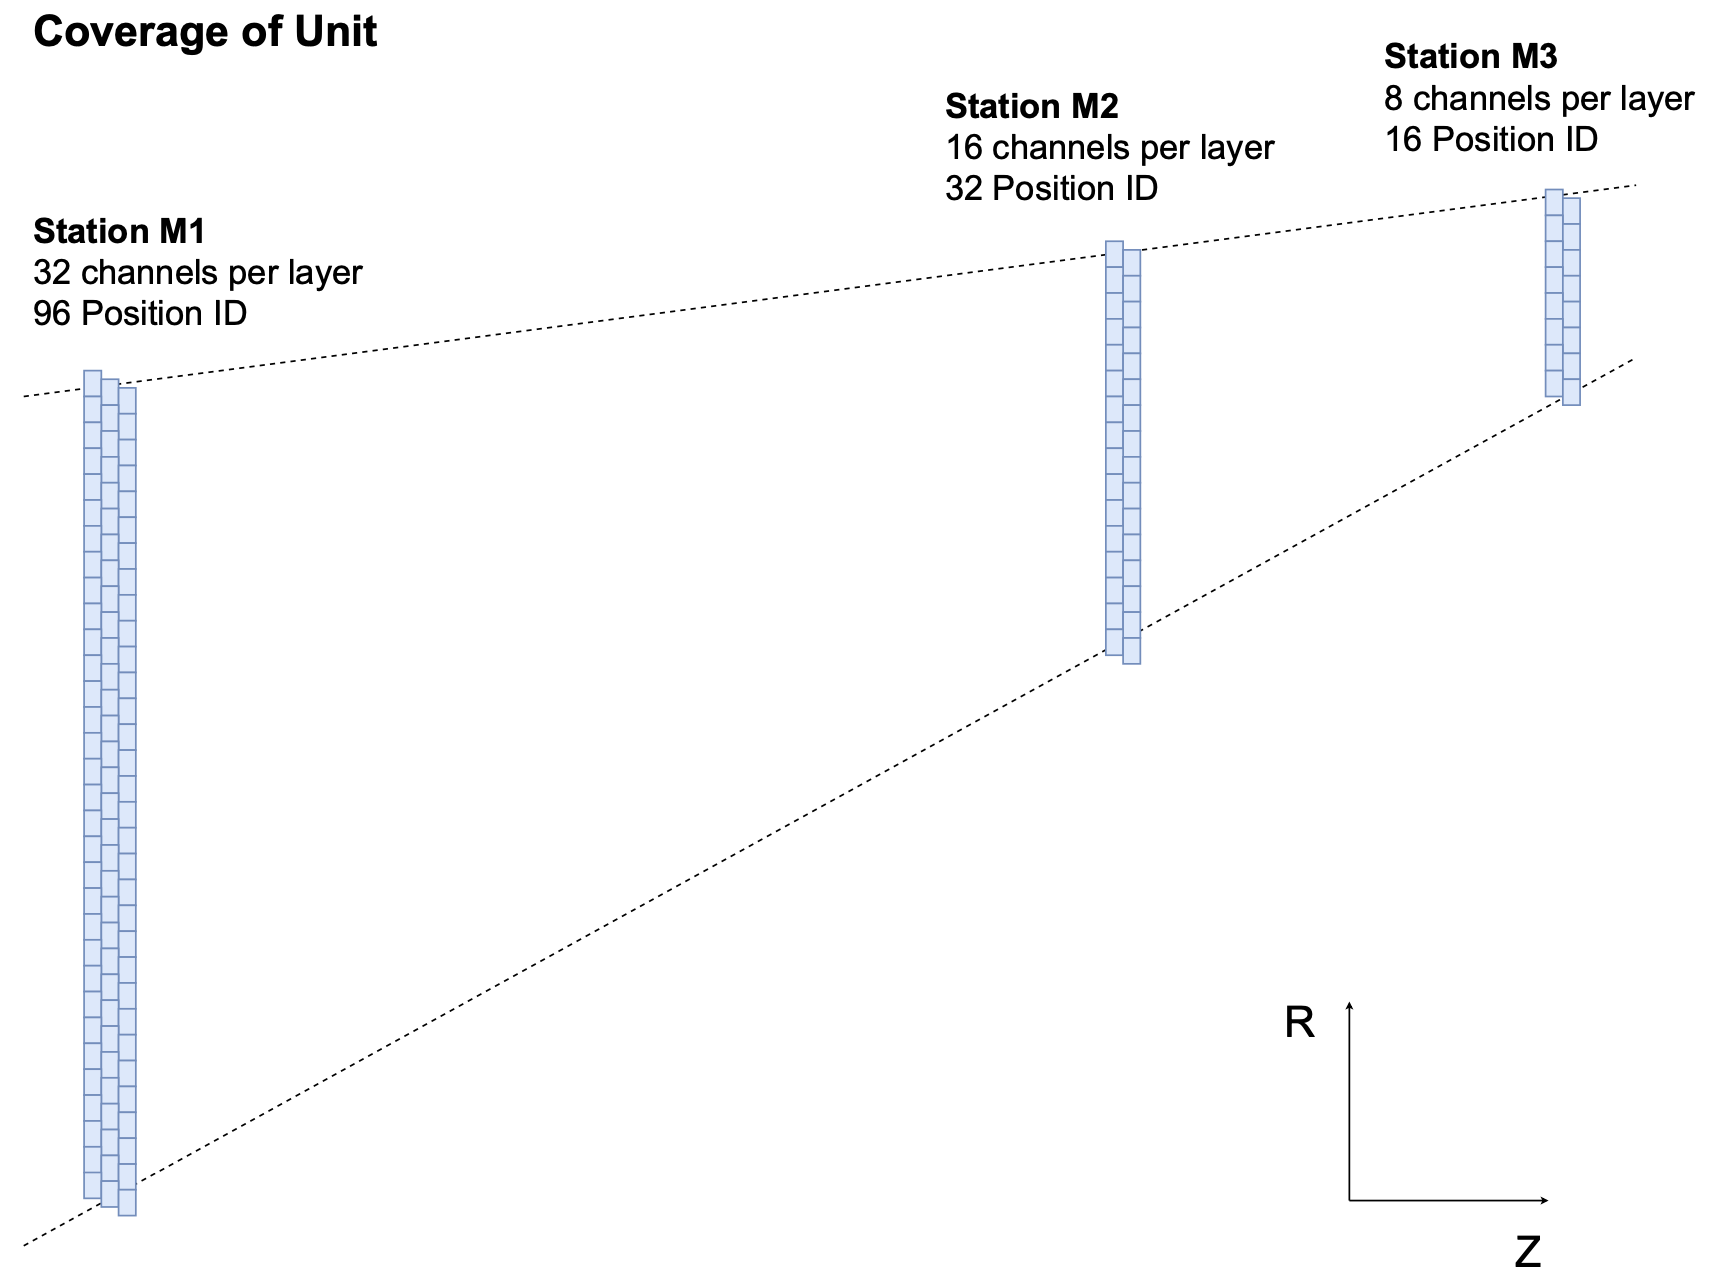
\includegraphics[width=0.8\textwidth]{figs/chapter5/wire_unit.png}
  \caption{Schematic of the coverage of a "Unit" region in three stations of wire segment reconstruction \cite{EndcapSLPDR}.}
  \label{fig:wire_unit}
\end{figure}

\subsubsection{Strip Segment Reconstruction}

Unlike the wire segment, for the strip segment, all three stations (M1, M2, and M3) are doublets and share symmetric geometry. so a single unified function is processing across all stations. Similar to the wire segments, \textit{Units} and \textit{Subunits} are also defined to structure the reconstruction process.

The strip segment reconstruction is divided into: 20, 20 and 4 Units in the Endcap 1, Endcap 2 and Forward region, respectively. Each Unit covers:
\begin{itemize}
  \item 8 strip channels per layer in M3,
  \item 12 strip channels per layer in M2,
  \item 20 strip channels per layer in M1.
\end{itemize}
And each strip Unit is subdivided into two \textit{Subunits}. Figure~\ref{fig:strip_unit} shows the coverage of a typical strip Unit.

The summary of coincidence type used in strip segment reconstrutction is shown as Table~\ref{tab:strip_coin}.
\begin{table}[htbp]
\centering
\small
\caption{Coincidence patterns for 6-layer strip segment reconstruction}
\label{tab:strip_coin}
\begin{tabular}{c|ccc}
\hline
\textbf{Coincidence pattern} & \textbf{M1} & \textbf{M2} & \textbf{M3} \\
\hline
6/6       & 2/2 & 2/2 & 2/2 \\
5/6 A     & 2/2 & 1/2 & 2/2 \\
5/6 B     & 1/2 & 2/2 & 2/2 \\
5/6 C     & 2/2 & 2/2 & 1/2 \\
4/6 A     & 1/2 & 1/2 & 2/2 \\
4/6 B     & 2/2 & 1/2 & 1/2 \\
4/6 C     & 1/2 & 2/2 & 1/2 \\
\hline
\end{tabular}
\end{table}

\begin{figure}[htbp]
  \centering
  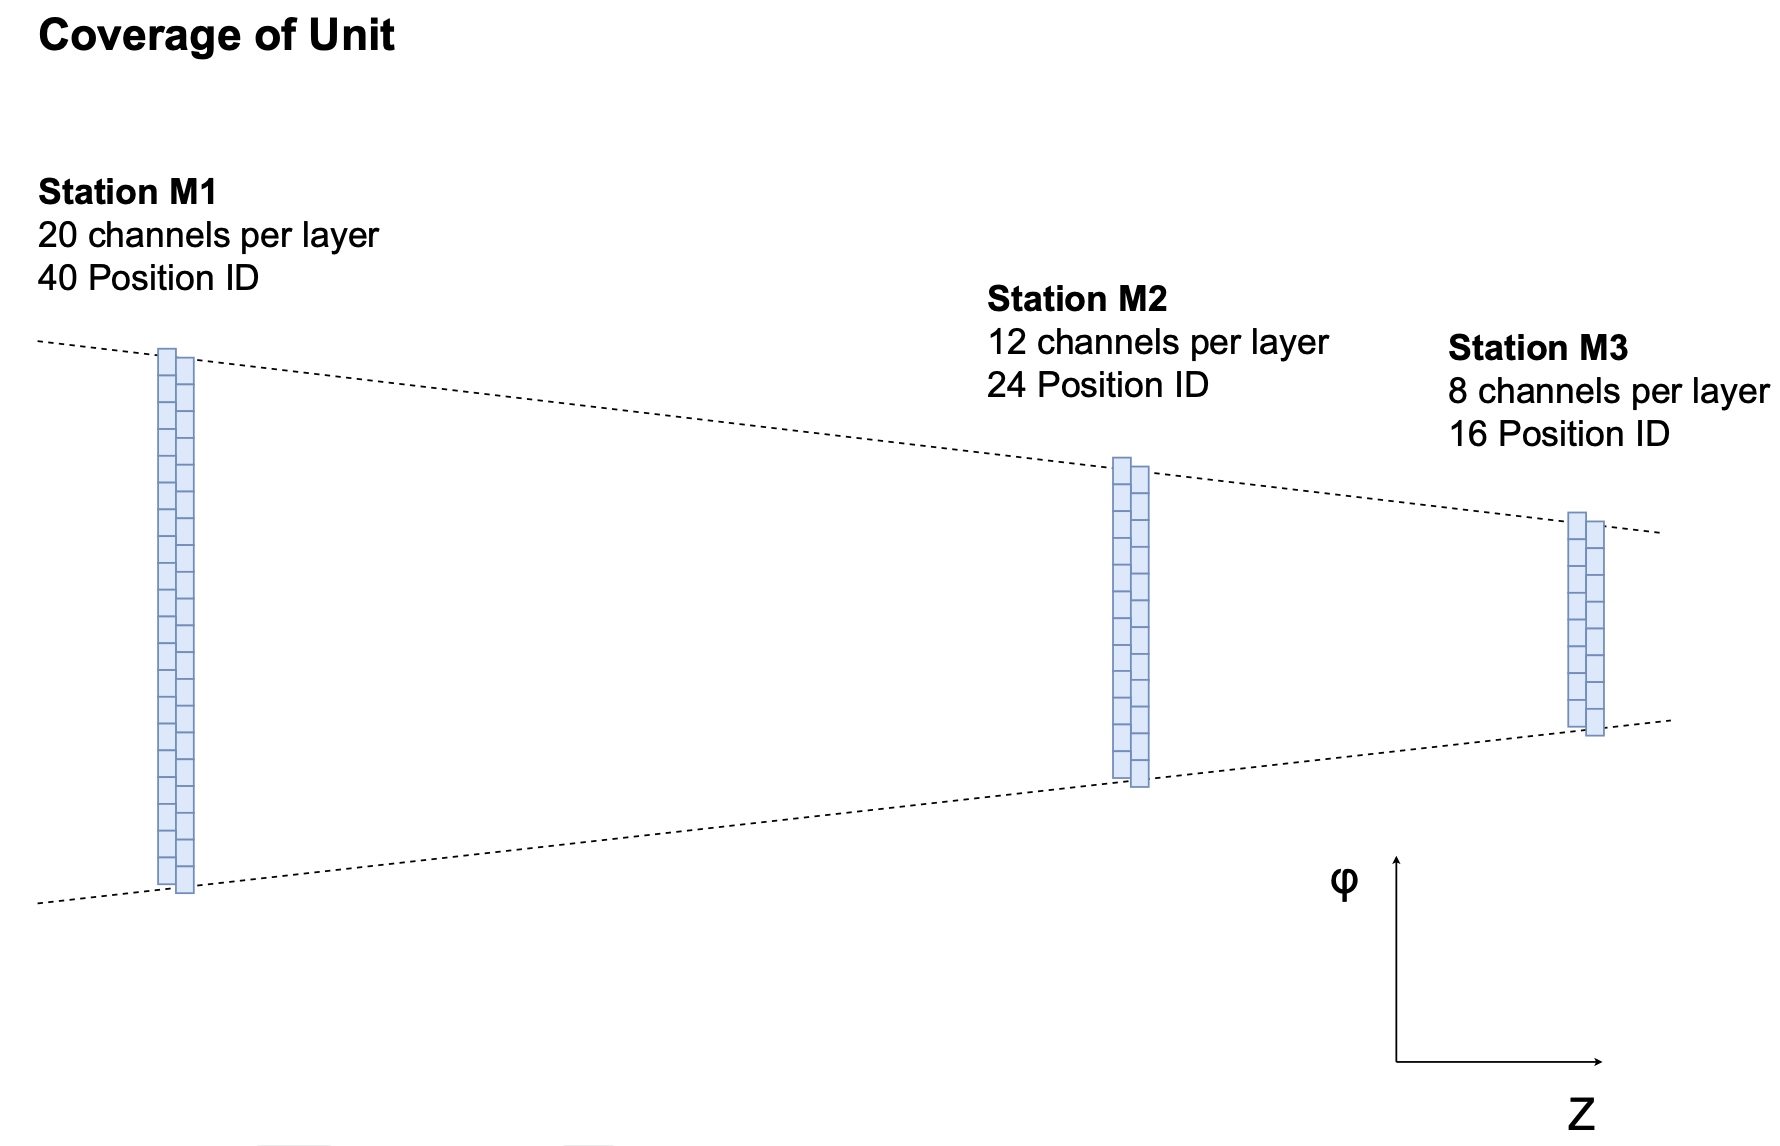
\includegraphics[width=0.8\textwidth]{figs/chapter5/strip_unit.png}
  \caption{Schematic of the coverage of a "Unit" region in three stations of strip segment reconstruction \cite{EndcapSLPDR}.}
  \label{fig:strip_unit}
\end{figure}

%====================================================================================================
\subsection{Wire-Strip Coincidence} \label{subsec:WireStripCoin}
%====================================================================================================
The Wire-Strip Coincidence is the final stage of reconstruction in the bitwise simulator. In this stage, the $\Delta\theta$ and $\Delta\phi$ values, along with the position information $\theta$ and $\phi$ from segment reconstruction are used to determine the transverse momentum ($p_{\mathrm{T}}$) of muons.

In the firmware, Wire-Strip Coincidence are divided into three parts, $p_{\mathrm{T}}$ Calculator, Wire Position Corrector, Block Seletor, which are processed parallelly. These components are all simulated in this simulator, arn are described below.

\subsubsection{$p_{\mathrm{T}}$ Calculator}

The previous obtained $\Delta\theta$ and $\Delta\phi$ are used to query a LUT determined by $\theta$ and $\phi$  to obtain the $p_{\mathrm{T}}$. The LUT used in this process is also referred as the \textit{Coincidence Window}, where $\Delta\theta$ is represented on the horizontal axis and $\Delta\phi$ on the vertical axis, and the value of $p_{\mathrm{T}}$ is encoded as a color corresponding to its magnitude. An schematic of this process is shown in Figure~\ref{fig:coin_window}.

\begin{figure}[htbp]
  \centering
  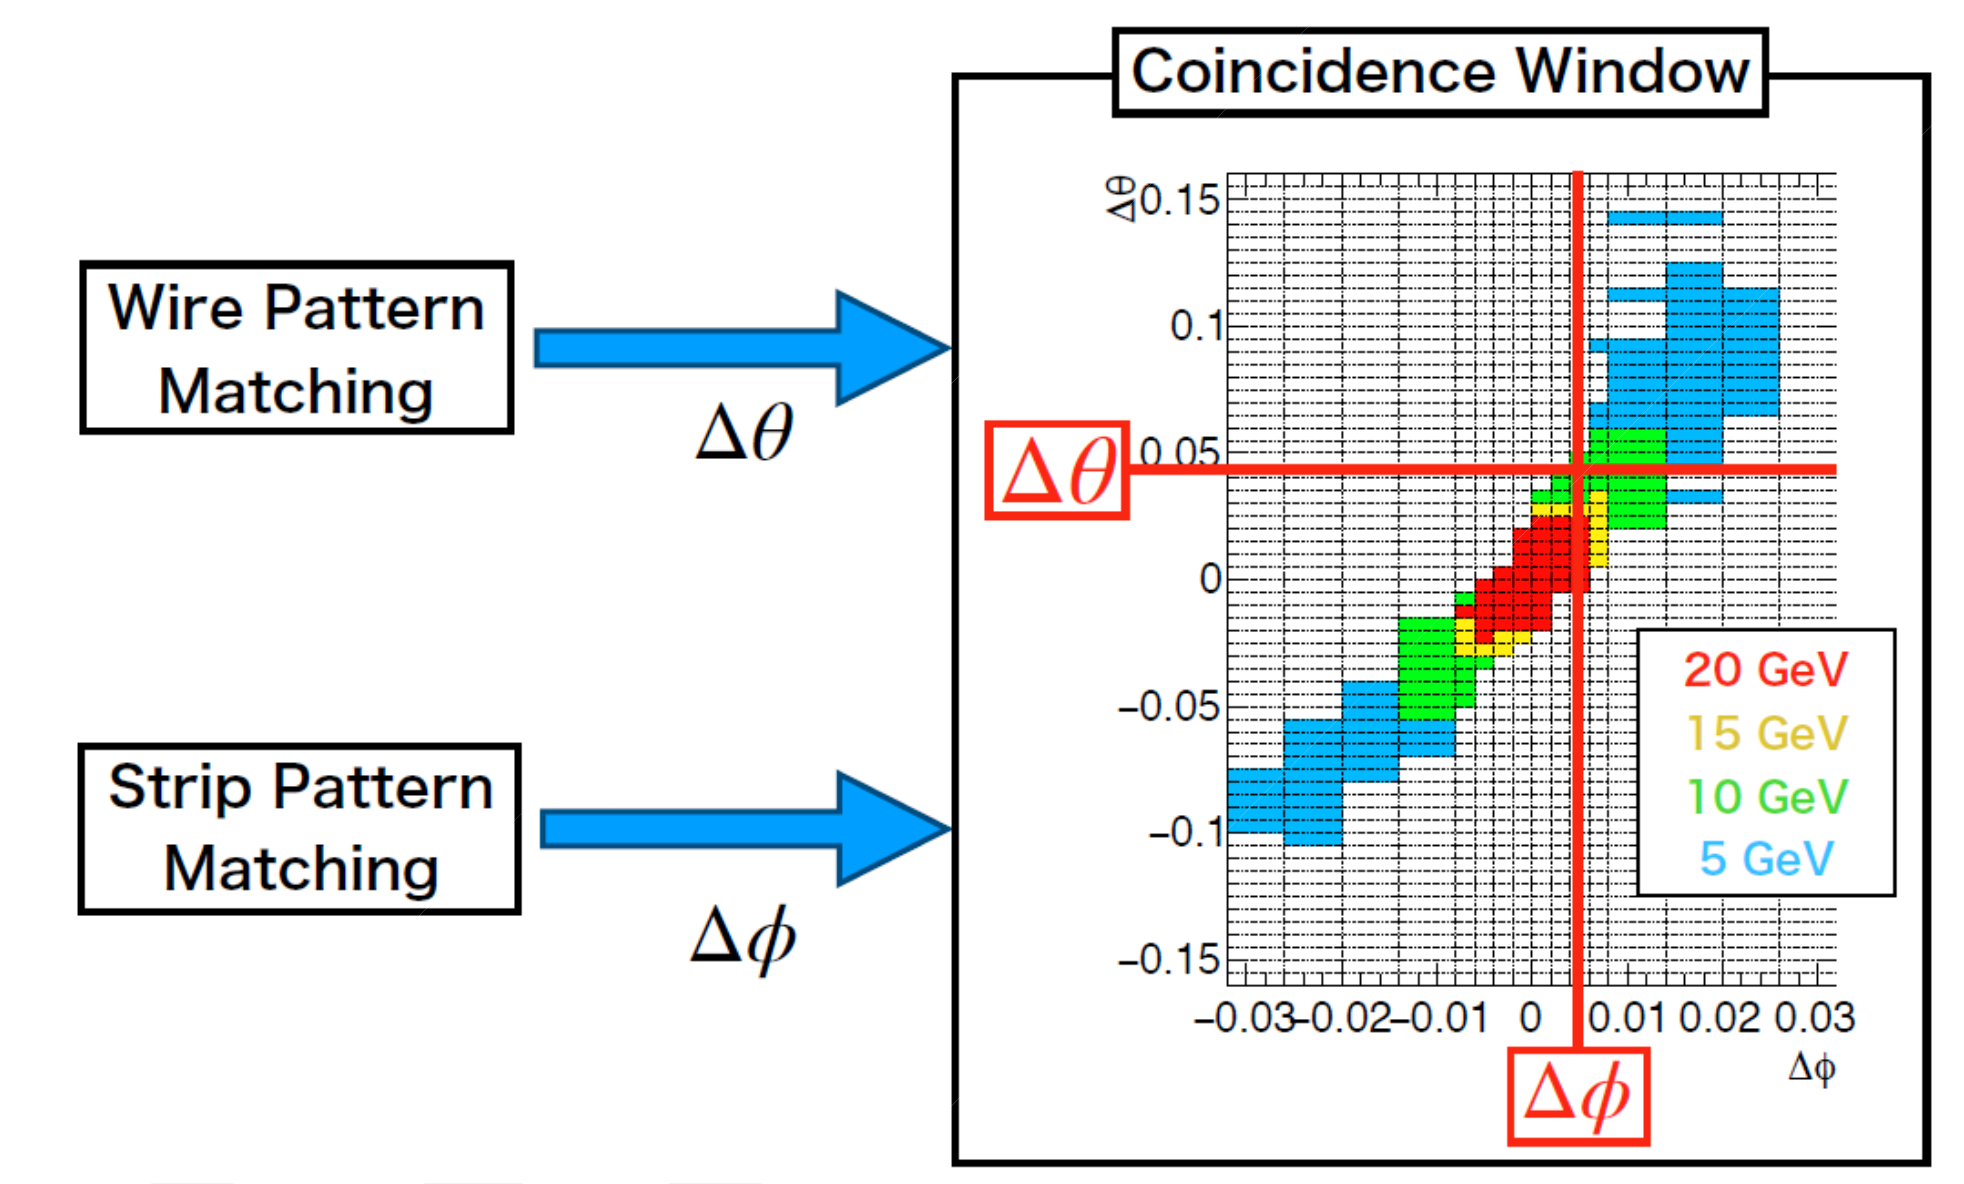
\includegraphics[width=1.0\textwidth]{figs/chapter5/coin_window.png}
  \caption{Schematic of $p_\mathrm{T}$ look-up process using Coincidence Window \cite{EndcapSLPDR}.}
  \label{fig:coin_window}
\end{figure}

In the firmware, the address for accessing the Coincidence Window (CW) in RAM consists of three components: 7 bits from the wire-side \(\Delta\theta\), 4 bits from the strip-side \(\Delta\phi\), and 2 bits indicating the URAM region number, making a total of 13 bits. Although the \(\Delta\theta\) and \(\Delta\phi\) values provided by the Segment Reconstruction module have widths of 8 bits and 9 bits, respectively, these are reduced to limit the size of the CW. For \(\Delta\theta\) of wire segment, the least significant bit is simply discarded, resulting in a 7-bit address input. For the strip side, \(\Delta\phi\), consisting of a 1-bit sign and an 8-bit absolute value, is nonlinearly compressed to 4 bits using the scheme in Table~\ref{tab:phi_encoding} to retain resolution near zero.

\begin{table}[htbp]
  \centering
  \caption{Mapping between 8-bit absolute value of input \(\Delta\phi\) and 3-bit compressed address value used in the $p_\mathrm{T}$ Calculator.}
  \label{tab:phi_encoding}
  \begin{tabular}{c|c}
    \hline
    Input \(\Delta\phi\) Absolute Value (8-bit) & Compressed Address Value (3-bit) \\
    \hline
    0--3     & Same as input (0--3) \\
    4--6     & 4 \\
    7--9     & 5 \\
    10--12   & 6 \\
    13 or more & 7 \\
    \hline
  \end{tabular}
\end{table}

As the output, the CW offers a 4-bit transverse momentum value. In the current implementation, five discrete output levels are defined: 0 (invalid), and 1–4 corresponding to transverse momentum thresholds of 5, 10, 15, and 20~GeV, respectively. To further improve precision, the development of a 16-stage CW is currently underway, as well as the application of machine learning techniques for CW generation.

\subsubsection{Block Selector}

The inputs to the Wire-Strip Coincidence consist of one wire information per \textit{subunit} and one strip information per \textit{unit}, the combination of the wire subunit and the strip unit is referred to as a \textit{block}. The Block Selector module evaluates these blocks within a specific so-called \textit{region}, using the angular information \((\Delta\phi, \Delta\theta)\) to determine which block within the region should be selected to output a valid \(p_{\mathrm{T}}\). The Block Selector operates independently of the pT Calculator and Wire Position Corrector, and thus performs a dedicated track reconstruction process that does not rely on the calculated \(p_{\mathrm{T}}\) value.

Two types of \textit{regions} are defined here: the \textit{8 Unit Region} and the \textit{32 Unit Region}. An 8 Unit Region consists of 2 wire subunits and 4 strip units, resulting in 8 block combinations. A 32 Unit Region, on the other hand, is composed of 8 wire subunits and 4 strip units, forming 32 possible blocks. As shown in Figure~\ref{fig:wsc_region}, in the endcap sectors \(\phi0\) and \(\phi1\), the region \(|\eta| < 1.3\) is covered by 22 instances of 8 Unit Regions, while the region \(|\eta| > 1.3\) is covered by 13 instances of 32 Unit Regions. In the forward region, 8 instances of 32 Unit Regions are used.

\begin{figure}[htbp]
  \centering
  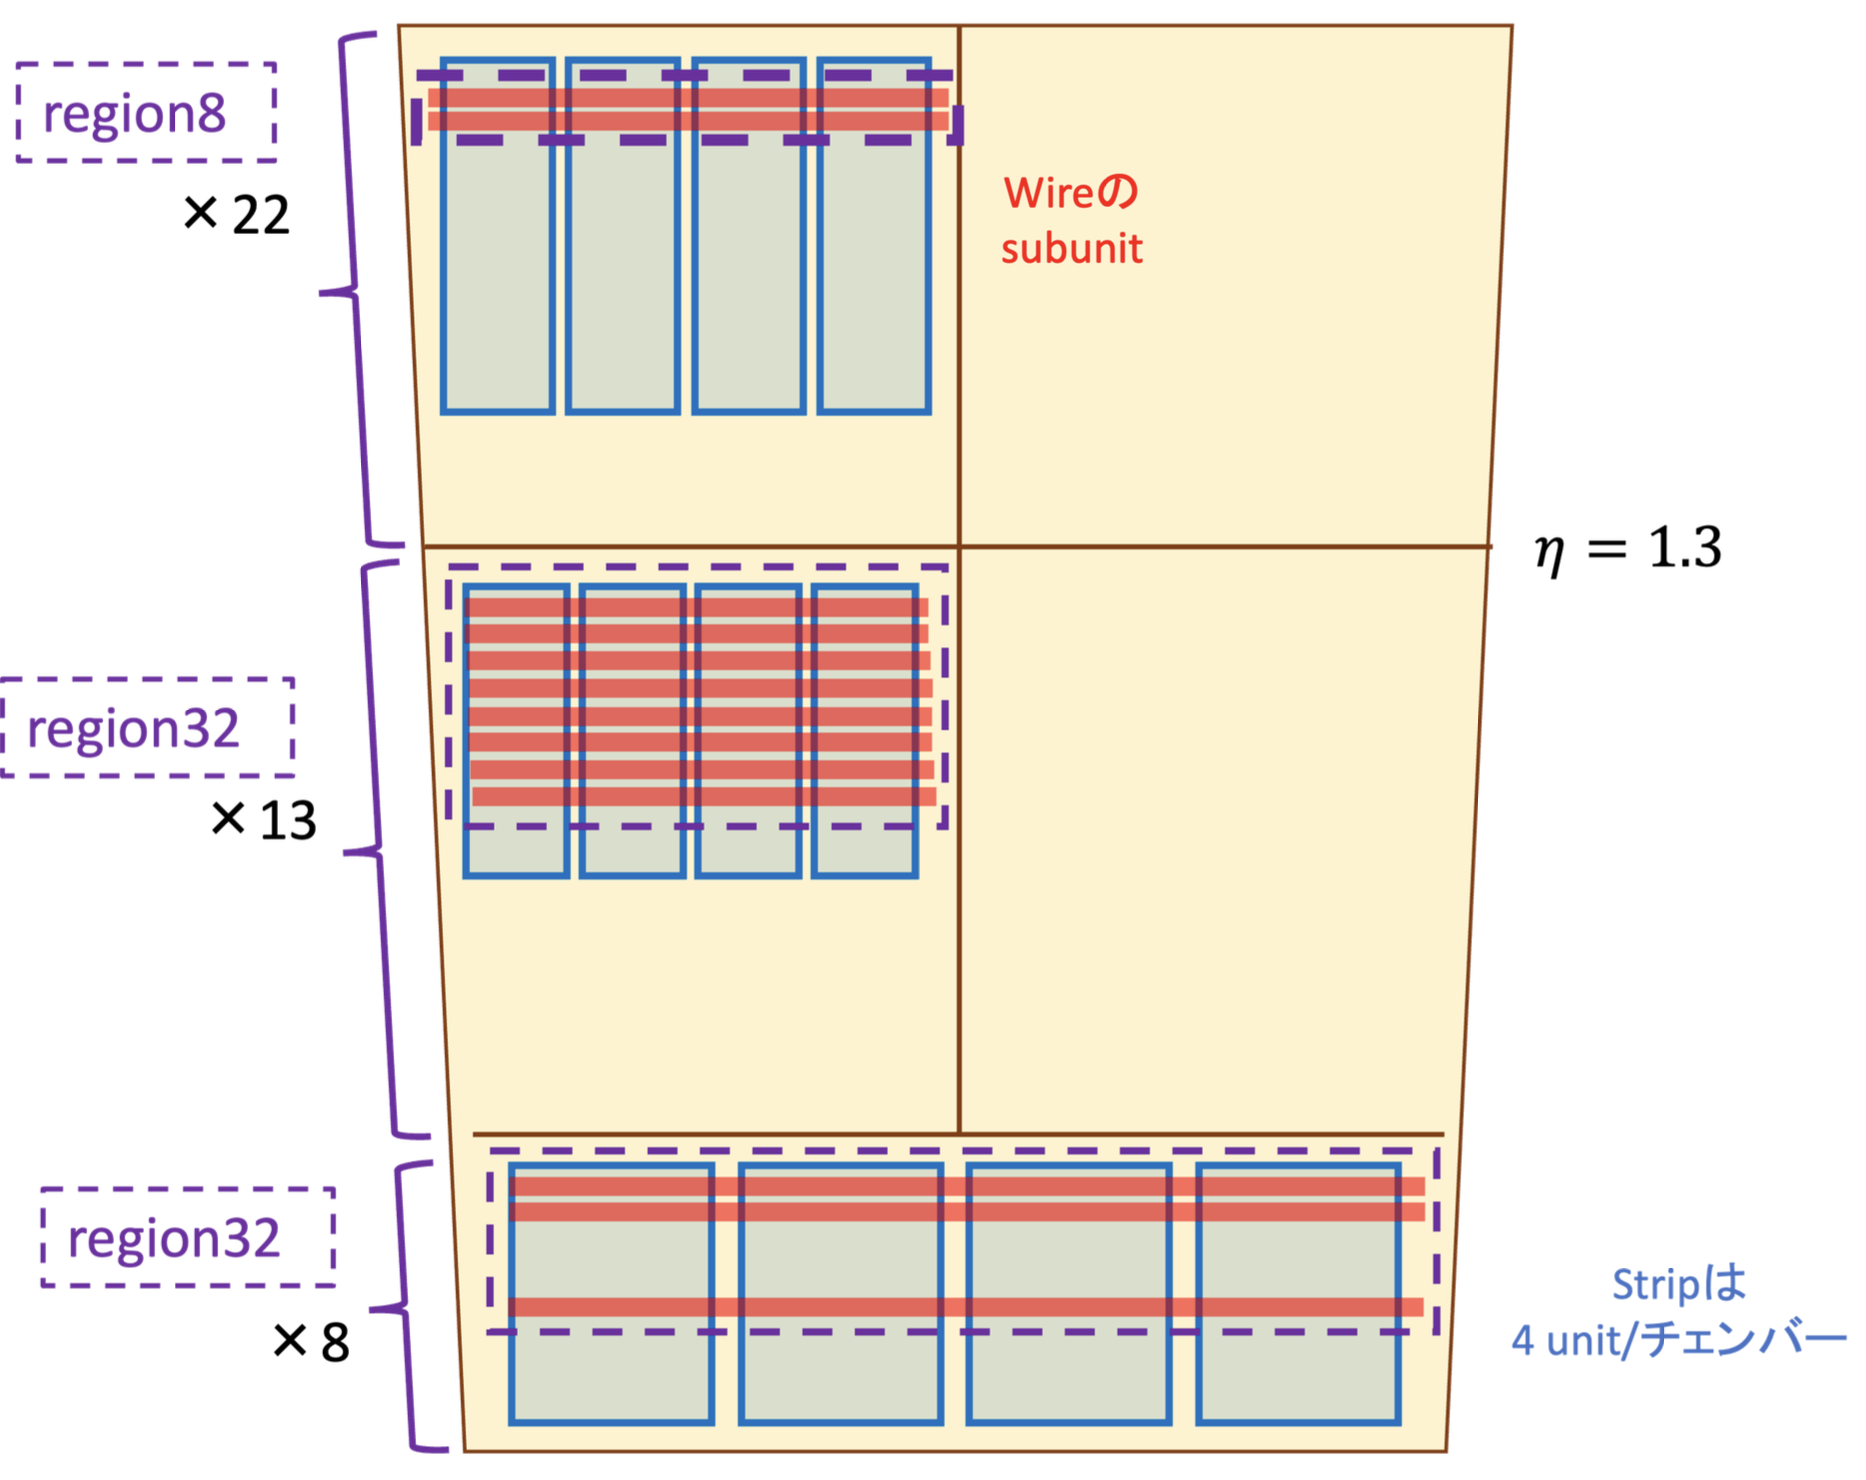
\includegraphics[width=1.0\textwidth]{figs/chapter5/wsc_region.png}
  \caption{Structure of 8 Unit Region (as "region8") and 32 Unit Region (as "region32") in Wire-Strip Coincidence \cite{yamashita}.}
  \label{fig:wsc_region}
\end{figure}

Within the Block Selector, wire and strip segments are reconstructed independently according to the following priority rules:
\begin{enumerate}
  \item Select the candidate with the most matched layers.
  \item If multiple candidates have the same number of matched layers, choose the one with the smaller angle.
\end{enumerate}

\paragraph{In an 8 Unit Region:}  
The region can contain up to 4 strip segments and 2 wire segments, yielding 8 possible block candidataes. Based on the priority logic, one strip segment and one wire segment are selected and combined to form a single output block candidate.

\paragraph{In a 32 Unit Region:}  
This region with larger $\eta$ may contain up to 4 strip segments and 8 wire segments, resulting in 32 possible block candidates. The Block Selector selects as below:
\begin{itemize}
  \item One wire segment with a positive angle, and one with a negative angle;
  \item Two strip segments.
\end{itemize}
As a result, $2 \times 2 = 4$ block candidates are selected in a 32 Unit Region.

\subsubsection{Wire Position Corrector}

The Wire Position Corrector is introduced to compensate for the geometric deviation in the reconstructed \(\eta\) coordinate caused by the linear sense wire structure of the wire segment. As is shown in Figure~\ref{fig:wire_corr}, the sense wire (anode wire) in the detector is arranged in straight lines, which do not align with the constant-\(\eta\) curves. Consequently, even for the same wire Position ID, the \(\eta\) value can vary depending on the associated reconstruction result in strip segment.

\begin{figure}[htbp]
  \centering
  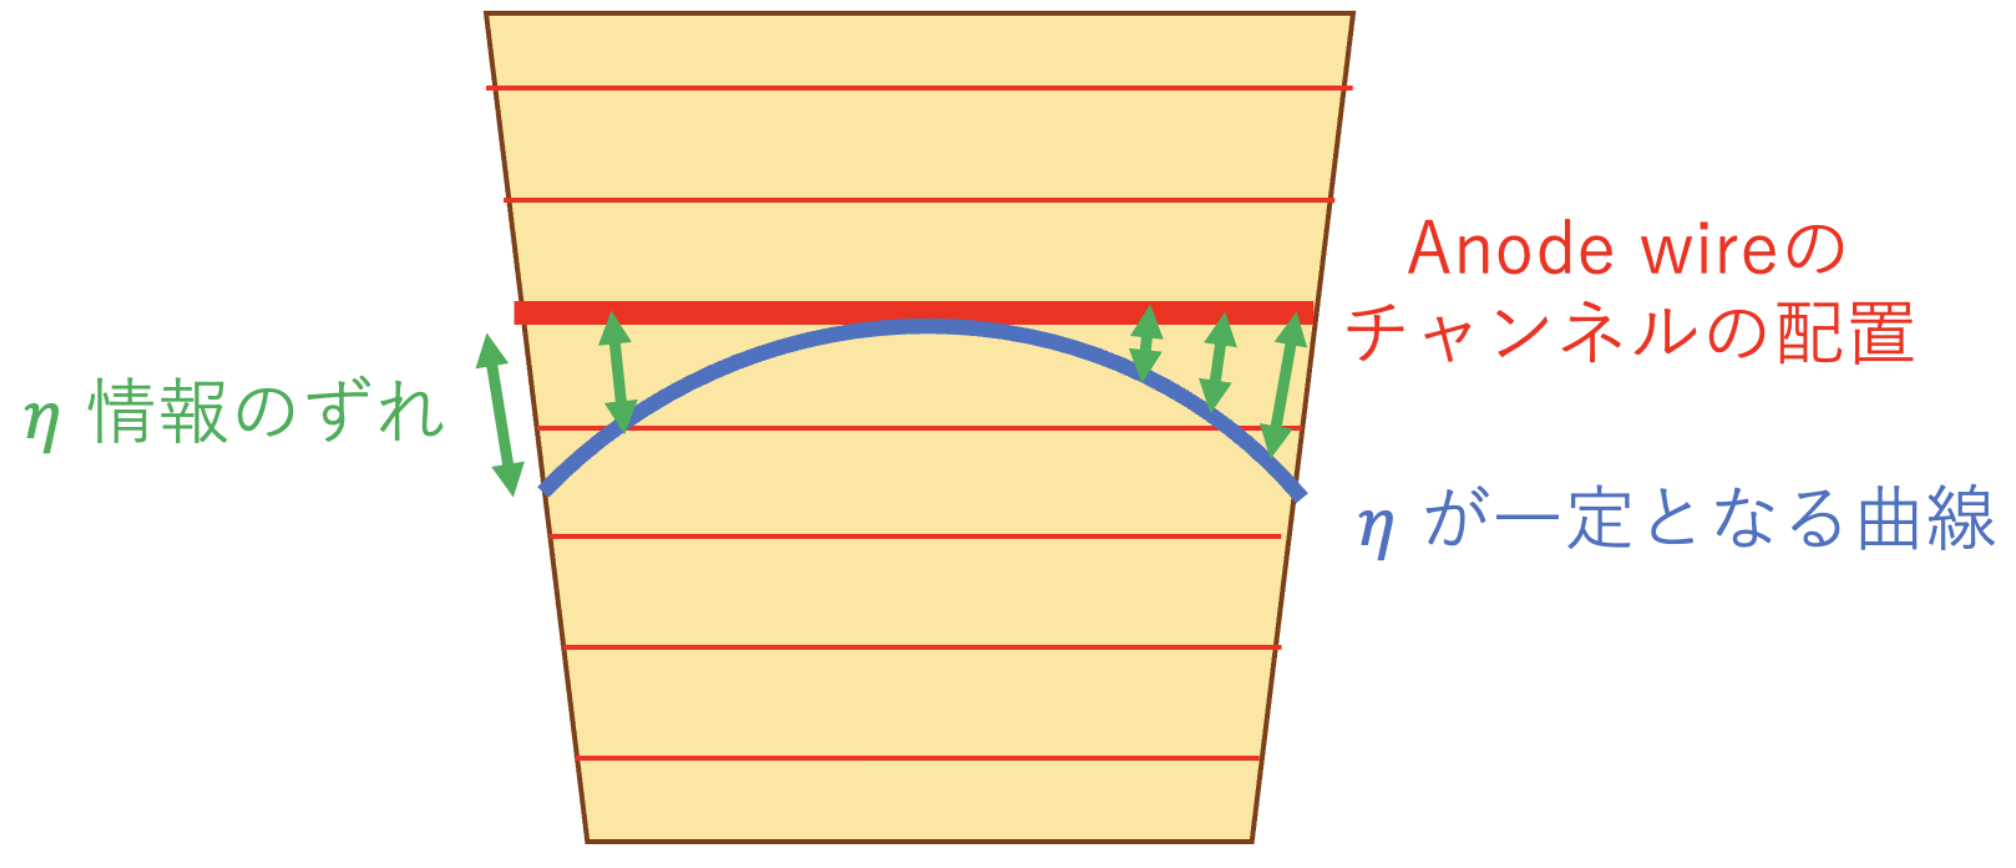
\includegraphics[width=1.0\textwidth]{figs/chapter5/wire_corr.png}
  \caption{Deviation between sense wire and constant-\(\eta\) curve \cite{yamashita}.}
  \label{fig:wire_corr}
\end{figure}

To correct this discrepancy, the bitwise Simulator refers to a dedicated Look-Up Table (LUT) that encodes the correspondence between the combination of wire and strip Position IDs and the true \(\eta\) coordinate. The LUT takes as input a 8-bit address, composed of the 2 bits from the wire Position ID and 6 bits from the strip Position ID. The output is an 8-bit corrected \(\eta\) value that is then attached to the reconstructed track.

%====================================================================================================
\section{Local Implementation on Athena} \label{sec:LocalImplementationOnAthena}
%====================================================================================================
This section describes the implementation of the bitwise simulator into the ATLAS software framework, Athena, which we briefly introduced in Chapter~\ref{ch:Athena}. The implementation work in this section is divided into two parts: 
First, the data input interface of the bitwise simulator was modified to conform to Athena's data flow and processing model. Second, the simulator, which originally handled only a single \(1/48\) TGC BW region, was extended to cover all sectors, including both A-side and C-side. This extension provides a testing environment for the Monte Carlo simulations described in the next chapter.
%====================================================================================================
\subsection{Input Adaptation for Athena} \label{subsec:InputAdaptation}
%====================================================================================================
The original bitwise simulator adopts bitmaps as its input format as it was designed to emulate the firmware behavior closely. While, the Athena-based implementation aims to simulate the trigger logic by Monte Carlo simulation samples as input. Specifically, the TGC simulation begins from RDO files generated by full detector simulation, from which TGC hit information is extracted in the form of \texttt{TgcDigit} containers. This section describes the unification of the input formats between the two simulators, allowing consistent application of the same trigger logic on Athena.

Figure~\ref{fig:input_adaptation} illustrates the forepart of data preparation and transformation steps for both the bitwise simulator and the Athena-based L0MuonS1TGCSimulator (hereafter referred to as L0TGCSimulator, which is the bitwise-Simulator-based simulator implemented on Athena). In the bitwise simulator, ROOT TTree files are used to store the hit bitmaps as initial input files, and then, the \textit{hitpattern operator}, as a dedicated tool, is used to convert ROOT tree files into vectors of boolean values representing the presence or absence of hits. These vectors are subsequently passed to the channel mapping module, as described in Section~\ref{subsec:ChannelMapping}, which converts them into structured vectors that encode hit information in terms of \textit{subsector}, \textit{layer}, and \textit{channel}.

\begin{figure}[htbp]
  \centering
  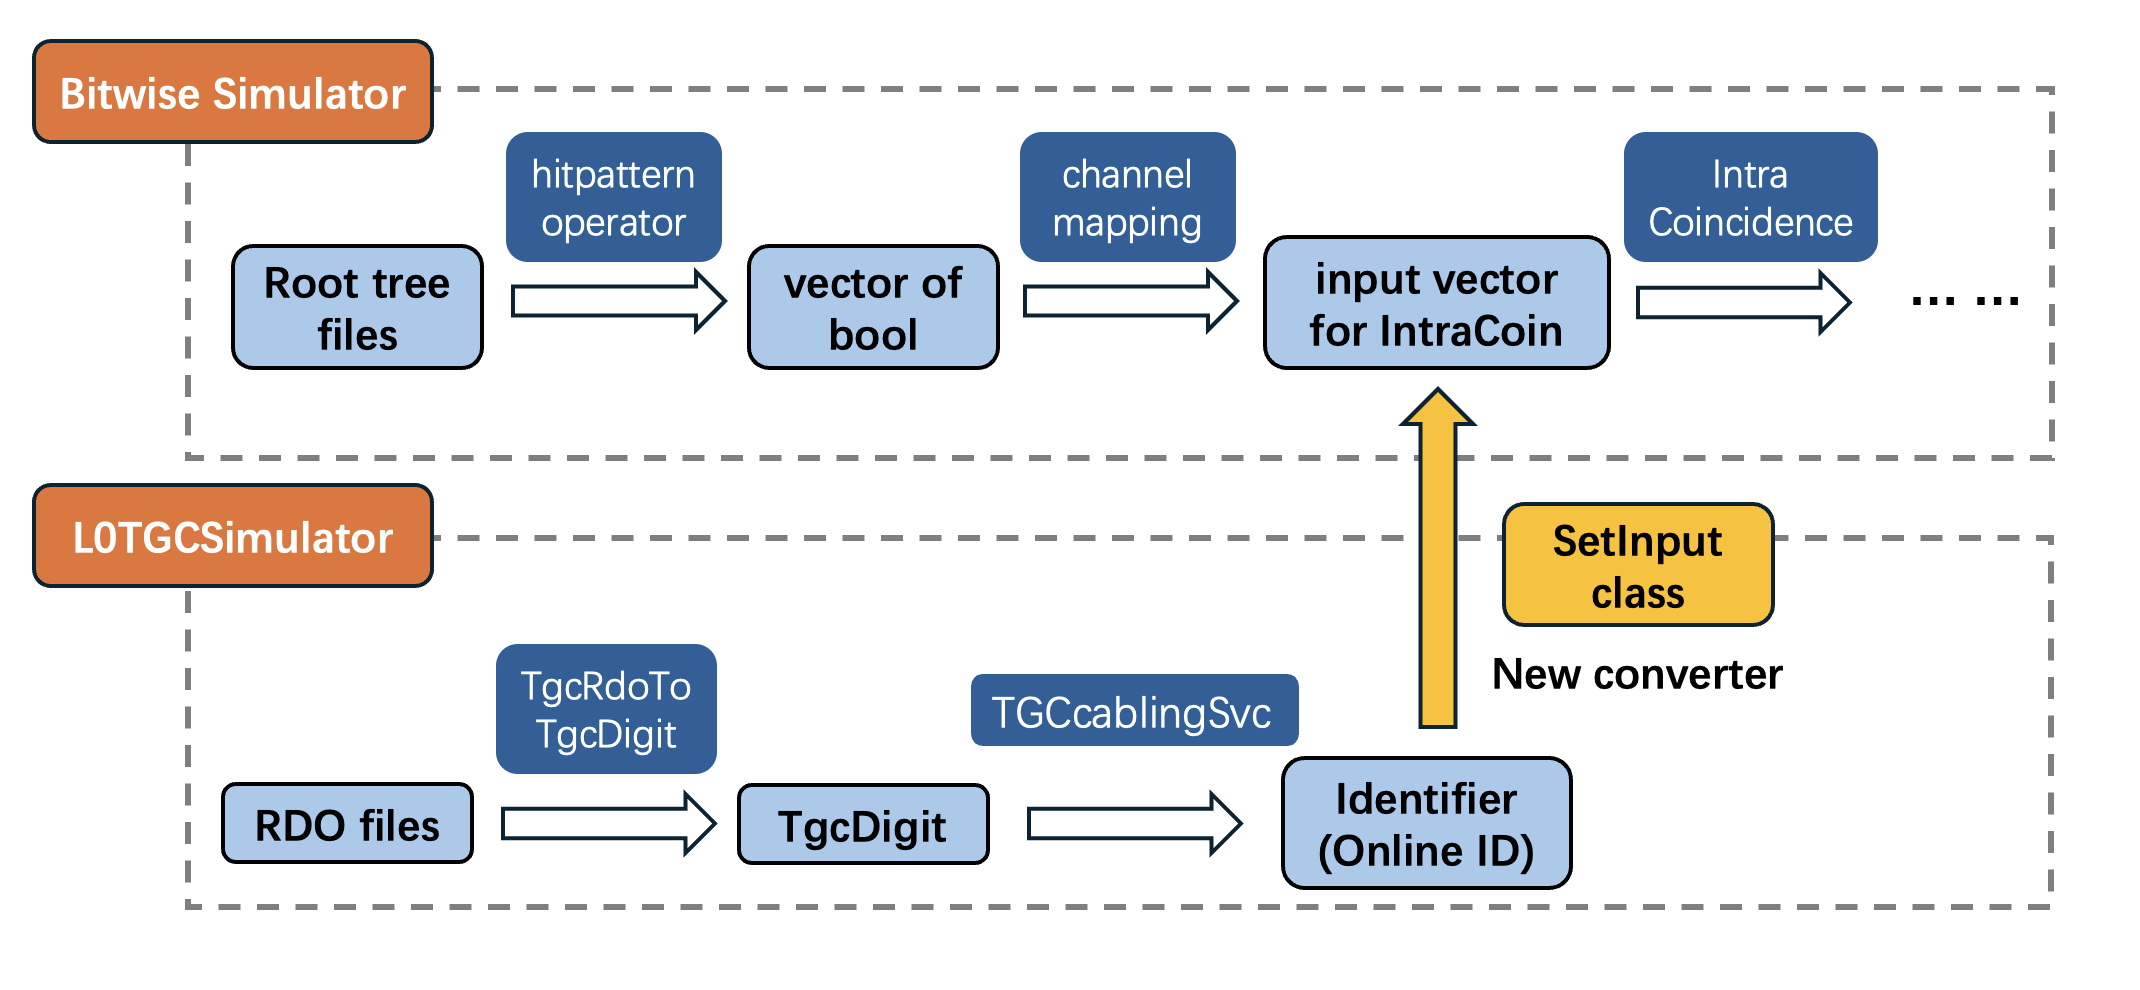
\includegraphics[width=1.0\textwidth]{figs/chapter5/input_adaptation.png}
  \caption{Illustration of the input adaptation process from the bitwise simulator to the L0TGCSimulator, enabled by the newly developed SetInput converter.}
  \label{fig:input_adaptation}
\end{figure}

The L0TGCSimulator receives as input the RDO files from simulation. First, the \\\texttt{TgcRdoToTgcDigitCfg} tool is used to extract data in \texttt{TgcDigit} format from the raw RDO data , which represents hit position information on the TGC detector. Then, the \texttt{m\_cabling} tool maps these \texttt{TgcDigits} into the Online ID format of the \textit{Identifier}, which is used to identify detector channels at the mechanical level. (The \textit{Identifier} currently supports four encoding schemes: Offline ID, Readout ID, Online ID, and Trigger ID. In this case, the Online ID format is used. For detailed explanations of the Identifier, please refer to the Appendix.) A summary of the structure and meaning of the Online ID is provided in Table~\ref{tab:OnlineID}.
\begin{table}[htbp]
  \centering
  \caption{List of variables in OnlineID}
  \label{tab:OnlineID}
  \begin{tabular}{|l|l|p{3cm}|p{6cm}|}
    \hline
    \textbf{Variable Name} & \textbf{Type} & \textbf{Value Range} & \textbf{Meaning} \\
    \hline
    subsystemNumber & int & A/C : +1/-1 & Indicates Aside or Cside \\
    \hline
    octantNumber & int & 0--7 & Index when dividing the wheel into 8 segments(3 sectors for each segments) in the increasing $\phi$ direction\\
    \hline
    moduleNumber & int & 0--12 & Identifier of each segment in increasing $\phi$ direction when dividing Endcap/Forward wheels into 8 parts (refer to Appendix)\\
    \hline
    layerNumber & int & 0--6: M1--M3;\newline 7,8: EI/FI & Index assigned to each layer in the increasing $z$ direction \\
    \hline
    rNumber & int & M1: 1--4;\newline M2,M3: 0--4;\newline Forward: 0 & Index assigned to each chamber in the increasing $\eta$ direction \\
    \hline
    wireOrStrip & bool & T/F: Strip/Wire & Distinction between Strip and Wire \\
    \hline
    channelNumber & int & 0--n & Logical channel number assigned to each channel \newline Wire: increases with $\eta$ \newline Strip: increases with $\phi$ \newline (AsideForward, CsideBackward) \newline decreases with $\phi$ \newline (AsideBackward, CsideForward) \\
    \hline
  \end{tabular}
\end{table}

To interface this with the trigger logic, I developed a class named \textit{SetInput} as shown in Figure~\ref{fig:input_adaptation}. This class receives the decoded Online IDs and converts them into the boolean input vectors required for the Intra Station Coincidence stage. The mapping rule between the Online ID values and the corresponding bit vector dimensions is described in Table~\ref{tab:OnlineID_vs_vector}.
\begin{table}[htbp]
  \centering
  \caption{Mapping Rule between the input vector dimensions and OnlineID}
  \label{tab:OnlineID_vs_vector}
  \begin{tabular}{|p{3cm}|p{4cm}|p{6cm}|}
    \hline
    \textbf{Indices of \newline Input Vector} & \textbf{OnlineID} & \textbf{Mapping Rule} \\
    \hline
    side & subsystemNumber & 0 for Aside ($+1$), 1 for Cside ($-1$) \\
    \hline
    sl & octantNumber,\newline moduleNumber & $sl = 3 \times$ octantNumber \newline $+ \lfloor$moduleNumber $/ 3\rfloor$ \\
    \hline
    subsec & moduleNumber & subsec = moduleNumber mod 3 \\
    \hline
    layer & layerNumber, isStrip & If Wire: layer = layerNumber \newline If Strip: layer = layerNumber + 6 \\
    \hline
    channel & channelNumber & same \\
    \hline
  \end{tabular}
\end{table}

%====================================================================================================
\subsection{Extension to All TGC Sectors} \label{subsec:Extension}
%====================================================================================================
Since the bitwise simulator was originally designed to simulate only 1/48 of the TGC Big Wheel (hereafter referred to as “one TGC sector”), in order to cover the complete endcap trigger logic and simulate muons across the entire endcap region, it is necessary to extend the bitwise simulator to all 48 TGC sectors of the BW (24 sectors on each of the A and C sides).

In the previous section, we described the adaptation of the \texttt{TgcDigit} input into the format used by the bitwise simulator for the Intra Station Coincidence logic. Since the Intra-Station Coincidence operates independently in each sector and follows the identical coincidence logic, I implemented the computation independently and in parallel for all TGC sectors, successfully achieving this part of the extension. In the following, we describe the extension of the subsequent processes: Wire/Strip Segment Reconstruction and Wire-Strip Coincidence (for convenience, we refer to these modules as IntraCoin, SegRec (WireRec and StripRec), and WSCoin hereafter, respectively.)

The modules \textit{SegRec} and \textit{WSCoin} rely on Look-Up Tables (LUTs) for the reconstruction process. Before performing the sector-wide extension of these modules, we first analyze the correspondence between LUTs and TGC sectors.

For \textit{SegRec}, one set of LUT are used for WireRec and StripRec respectively. In the \textit{WSCoin} process, due to the presence of the Wire Segment Corrector, two set of LUTs are required: one for transverse momentum ($p_\mathrm{T}$) calculation, and another for $\eta$ correction of the wire segment. Taking into account the $\phi$-dependent geometry of each sector and the inherent symmetry across sectors, it is determined that a single shared LUT can be used for all 24 sectors on one side (Aside or Cside) for WireRec, StripRec, and the Wire Segment Corrector. However, the $p_\mathrm{T}$ LUT (referred to as WSPattern) follows a cyclical pattern across sectors: every three adjacent sectors use distinct LUTs, and this pattern repeats eight times within each side.

The correspondence between LUT types and TGC sectors is summarized in Table~\ref{tab:LUT_with_sectors}.
\begin{table}[htbp]
  \centering
  \caption{LUT types and their sector-wise application strategy}
  \label{tab:LUT_with_sectors}
  \begin{tabular}{|c|p{8cm}|}
    \hline
    \textbf{LUT Type} & \textbf{LUT-Sectors Mapping Strategy} \\
    \hline
    WireRec LUT & Shared across all sectors on one side \\
    \hline
    StripRec LUT & Shared across all sectors on one side  \\
    \hline
    WSPattern LUT & 3-sector cyclic pattern repeated 8 times on one side (see Figure~\ref{fig:LUT_sharing}) \\
    \hline
    WCorrPattern LUT & Shared across all sectors on one side  \\
    \hline
  \end{tabular}
\end{table}

Following a similar approach to the \textit{IntraCoin} extension, we defined one object per sector for \textit{WireRec}, \textit{StripRec} and \textit{WSCoin}, and each object is assigned the corresponding LUT according to its sector position. The output results confirm that the reconstruction is processing successfully across all 48 TGC sectors. Further evaluations are performed in Chapter~\ref{ch:PerformanceEvaluation}.
%====================================================================================================
\section{Memory Reduction of LUT} \label{MemoryReduction}
%====================================================================================================
In the previous section, the bitwise simulator was successfully integrated into Athena and verified to run locally. However, to support future integration into the authentic Athena environment, it is essential to reduce the simulator's memory usage to meet the framework’s memory constraints, which is around 500 \text{MB} for the simulation of TGC detector.

Analysis of the original bitwise simulator shows that a single-sector instance occupies approximately 296 \text{MB} of memory. If directly scaled to cover all 48 TGC sectors, the total memory usage would reach
\[
48 \times 296 \text{MB} \simeq 14 \text{GB},
\]
which significantly exceeds the permissible limit. Through the optimisation strategies described in this section, the extended L0TGCSimulator reduces total memory usage to approximately 6.3 \text{GB}.

The LUTs used in the Segment Reconstruction and Wire–Strip Coincidence modules, which are main processes of the simulator, consumes a large quantity of memory usage. These LUTs are responsible for reconstructing $\Delta\theta$, $\Delta\phi$, and $p_{\mathrm{T}}$, and are stored using high-dimensional vectors and \textit{map} variable to emulate the address hierarchy of the URAM in firmware. Each vector dimension corresponds to the pivot hit position information, which is used to locate the LUT (this position information indicates the corresponding \textit{subunit} position of hit on M3 station in SegRec, and the $\eta$ value of the M3 hit in WSCoin). 

In the bitwise simulator before implementation, any index as dimension only uses lower than 6 bits in value, however stored within a 32 bit integer, resulting in vast amounts of unused address space. This inefficiency is visualised on the left side of Fig.~\ref{fig:LUT_optimization}, which abstracts the LUT container into a three-dimensional cube.
\begin{figure}[htbp]
  \centering
  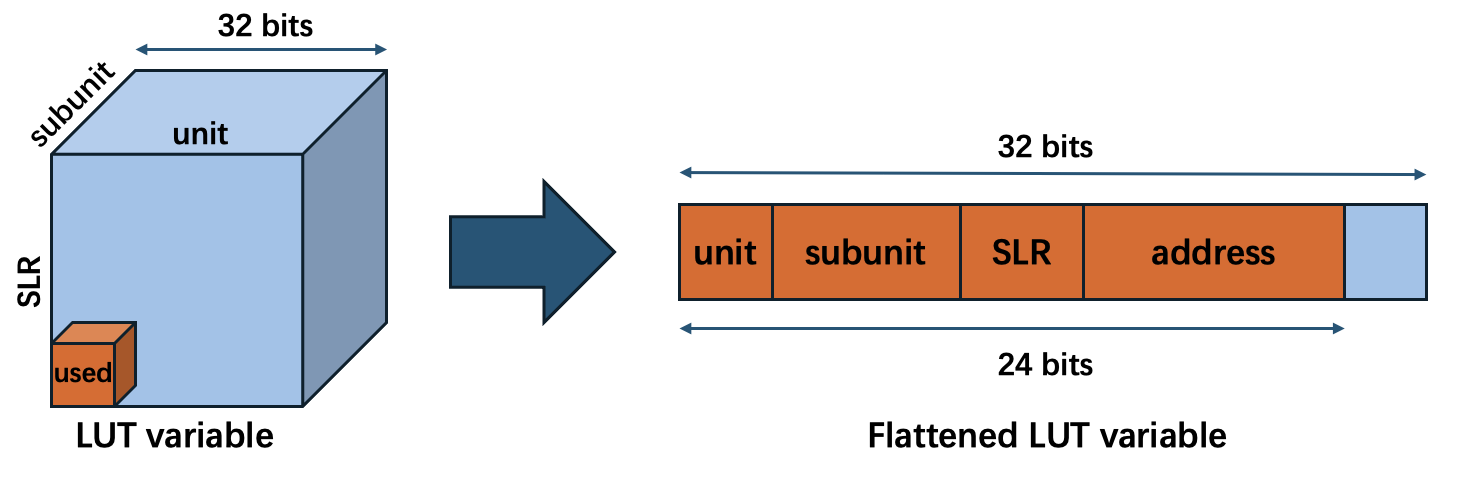
\includegraphics[width=1.0\textwidth]{figs/chapter5/LUT_optimization.png}
  \caption{Illustration of the LUT optimization strategy. The left part shows the high-dimensional vectors storing way, while the right one demonstrates the storing after flattening technique.}
  \label{fig:LUT_optimization}
\end{figure}

To address this, a new strategy was performed that flattens the multi-dimensional container into a one-dimensional map by packing the individual coordinate indices into a single integer key as \textit{uint}. Each field uses only as many bits as required by its range, and the final key is constructed through bit-shifting. The result is a more compact and efficient memory structure, as shown in the right part of Fig.~\ref{fig:LUT_optimization}. An illustrative overview of the new LUT structure is shown in Table~\ref{tab:LUT_store_structure}. All four LUT types—SegRecWire, SegRecStrip, WSPattern, and Wire Segment Corrector—were migrated to this representation.
\begin{table}[htbp]
  \centering
  \caption{Bit-level structure of key and value for each LUT in the simulator}
  \label{tab:LUT_store_structure}
  
  %---------------- Segment Rec Wire ----------------
  \begin{tabular}{|p{4.5cm}|p{1cm}|p{1cm}|p{2cm}|p{1cm}|p{1cm}|p{1cm}|}
    \hline
    \texttt{m\_map\_SegRecWire\_LUTs} & SLR & unit & subunit & i & key & value \\
    \hline
    bits & 2 & 6 & 2 & 2 & 12 & 18 \\
    \hline
    sum & \multicolumn{6}{c|}{24-bit key, 18-bit value} \\
    \hline
  \end{tabular}
  \vspace{0.5em}

  %---------------- Segment Rec Strip ----------------
  \begin{tabular}{|p{4.5cm}|p{1cm}|p{1.6cm}|p{1cm}|p{1.5cm}|p{0.9cm}|p{1cm}|}
    \hline
    \texttt{m\_map\_SegRecStrip\_LUTs} & SLR & ichamber & iuram & isUramB & key & value \\
    \hline
    bits & 2 & 3 & 2 & 1 & 16 & 9 \\
    \hline
    sum & \multicolumn{6}{c|}{24-bit key, 9-bit value} \\
    \hline
  \end{tabular}
  \vspace{0.5em}

  %---------------- WSPattern ----------------
  \begin{tabular}{|p{4.5cm}|p{3cm}|p{3cm}|p{1cm}|}
    \hline
    \texttt{m\_WSPattern\_map} & eta\_ID & address & value \\
    \hline
    bits & 16 & 16 & 4 \\
    \hline
    sum & \multicolumn{3}{c|}{32-bit key, 4-bit value} \\
    \hline
  \end{tabular}
  \vspace{0.5em}

  %---------------- WCorr ----------------
  \begin{tabular}{|p{4.5cm}|p{3cm}|p{3cm}|p{1cm}|}
    \hline
    \texttt{m\_WCorrPattern\_map} & eta\_ID & address & value \\
    \hline
    bits & 16 & 8 & 1 \\
    \hline
    sum & \multicolumn{3}{c|}{24-bit key, 1-bit value} \\
    \hline
  \end{tabular}
  \vspace{0.5em}
\end{table}



To further optimise both memory and access time, the standard \texttt{std::map} container was replaced by \texttt{std::unordered\_map}. A \texttt{std::map} in C++ is an associative container that stores key-value pairs in a sorted order according to the key. Internally, it uses a self-balancing binary search tree (BST), like a Red-Black tree. This guarantees logarithmic time complexity $\mathcal{O}(\log n)$ for insertion, deletion, and search operations. On the other hand, \texttt{std::unordered\_map} is implemented using a \textit{hash table}. This allows average constant-time complexity $\mathcal{O}(1)$ for insertion, deletion, and lookup, though the element order is not maintained. Because it avoids tree-based structures, it also consumes less memory on average. In the present case, since the keys used to represent hit patterns stored in the LUT are typically sparse and discontinuous, using a unordered\_map is suited to this purpose and does not cause problems. The main differences between map and unordered\_map are listed in Table~\ref{tab:map_vs_unorderedmap}.
\begin{table}[htbp]
  \centering
  \caption{Comparison between \texttt{std::map} and \texttt{std::unordered\_map} in C++}
  \label{tab:map_vs_unorderedmap}
  \begin{tabular}{|l|l|p{5.5cm}|}
    \hline
    \textbf{Feature} & \texttt{std::map} & \texttt{std::unordered\_map} \\
    \hline
    Data Structure & Self-balancing BST & Hash Table \\
    \hline
    Order & Sorted order & No specific order \\
    \hline
    Time Complexity & $\mathcal{O}(\log n)$ & $\mathcal{O}(1)$ on average \\
    \hline
    Memory Usage & Higher (due to tree nodes) & Lower (uses hashing) \\
    \hline
    Use Case & When sorted order is required & When order is unimportant but speed is crucial \\
    \hline
  \end{tabular}
\end{table}

The final data structures used are as follows: the sizes of "uint" variables are adjusted by the numbers of necessary bits of address and position information.
\begin{itemize}
  \item \texttt{std::unordered\_map<uint32\_t, uint32\_t>} for WireRec LUTs;
  \item \texttt{std::unordered\_map<uint32\_t, uint32\_t>} for StripRec LUTs;
  \item \texttt{std::unordered\_map<uint32\_t, uint8\_t>}  for WSPattern LUTs;
  \item \texttt{std::unordered\_map<uint32\_t, uint8\_t>}  for WCorr LUTs.
\end{itemize}

As a result of these optimisations, the memory required for a single-sector bitwise simulator was reduced from 296 \text{MB} to 260 \text{MB}, a reduction of approximately 12\%. Additionally, during the integration, a one-time full loading strategy was adopted for all LUTs at initialization, in contrast to the original bitwise simulator which rewrote LUT content upon each use. Combined with the LUT sharing across sectors on the same side discussed earlier, this contributed further to the reduction of the total memory of the implemented L0TGCSimulator, from the originally estimated 14 \text{GB} down to approximately 6.3 \text{GB}.
